% Options for packages loaded elsewhere
% Options for packages loaded elsewhere
\PassOptionsToPackage{unicode}{hyperref}
\PassOptionsToPackage{hyphens}{url}
\PassOptionsToPackage{dvipsnames,svgnames,x11names}{xcolor}
%
\documentclass[
  letterpaper,
  DIV=11,
  numbers=noendperiod]{scrartcl}
\usepackage{xcolor}
\usepackage{amsmath,amssymb}
\setcounter{secnumdepth}{5}
\usepackage{iftex}
\ifPDFTeX
  \usepackage[T1]{fontenc}
  \usepackage[utf8]{inputenc}
  \usepackage{textcomp} % provide euro and other symbols
\else % if luatex or xetex
  \usepackage{unicode-math} % this also loads fontspec
  \defaultfontfeatures{Scale=MatchLowercase}
  \defaultfontfeatures[\rmfamily]{Ligatures=TeX,Scale=1}
\fi
\usepackage{lmodern}
\ifPDFTeX\else
  % xetex/luatex font selection
\fi
% Use upquote if available, for straight quotes in verbatim environments
\IfFileExists{upquote.sty}{\usepackage{upquote}}{}
\IfFileExists{microtype.sty}{% use microtype if available
  \usepackage[]{microtype}
  \UseMicrotypeSet[protrusion]{basicmath} % disable protrusion for tt fonts
}{}
\makeatletter
\@ifundefined{KOMAClassName}{% if non-KOMA class
  \IfFileExists{parskip.sty}{%
    \usepackage{parskip}
  }{% else
    \setlength{\parindent}{0pt}
    \setlength{\parskip}{6pt plus 2pt minus 1pt}}
}{% if KOMA class
  \KOMAoptions{parskip=half}}
\makeatother
% Make \paragraph and \subparagraph free-standing
\makeatletter
\ifx\paragraph\undefined\else
  \let\oldparagraph\paragraph
  \renewcommand{\paragraph}{
    \@ifstar
      \xxxParagraphStar
      \xxxParagraphNoStar
  }
  \newcommand{\xxxParagraphStar}[1]{\oldparagraph*{#1}\mbox{}}
  \newcommand{\xxxParagraphNoStar}[1]{\oldparagraph{#1}\mbox{}}
\fi
\ifx\subparagraph\undefined\else
  \let\oldsubparagraph\subparagraph
  \renewcommand{\subparagraph}{
    \@ifstar
      \xxxSubParagraphStar
      \xxxSubParagraphNoStar
  }
  \newcommand{\xxxSubParagraphStar}[1]{\oldsubparagraph*{#1}\mbox{}}
  \newcommand{\xxxSubParagraphNoStar}[1]{\oldsubparagraph{#1}\mbox{}}
\fi
\makeatother

\usepackage{color}
\usepackage{fancyvrb}
\newcommand{\VerbBar}{|}
\newcommand{\VERB}{\Verb[commandchars=\\\{\}]}
\DefineVerbatimEnvironment{Highlighting}{Verbatim}{commandchars=\\\{\}}
% Add ',fontsize=\small' for more characters per line
\usepackage{framed}
\definecolor{shadecolor}{RGB}{241,243,245}
\newenvironment{Shaded}{\begin{snugshade}}{\end{snugshade}}
\newcommand{\AlertTok}[1]{\textcolor[rgb]{0.68,0.00,0.00}{#1}}
\newcommand{\AnnotationTok}[1]{\textcolor[rgb]{0.37,0.37,0.37}{#1}}
\newcommand{\AttributeTok}[1]{\textcolor[rgb]{0.40,0.45,0.13}{#1}}
\newcommand{\BaseNTok}[1]{\textcolor[rgb]{0.68,0.00,0.00}{#1}}
\newcommand{\BuiltInTok}[1]{\textcolor[rgb]{0.00,0.23,0.31}{#1}}
\newcommand{\CharTok}[1]{\textcolor[rgb]{0.13,0.47,0.30}{#1}}
\newcommand{\CommentTok}[1]{\textcolor[rgb]{0.37,0.37,0.37}{#1}}
\newcommand{\CommentVarTok}[1]{\textcolor[rgb]{0.37,0.37,0.37}{\textit{#1}}}
\newcommand{\ConstantTok}[1]{\textcolor[rgb]{0.56,0.35,0.01}{#1}}
\newcommand{\ControlFlowTok}[1]{\textcolor[rgb]{0.00,0.23,0.31}{\textbf{#1}}}
\newcommand{\DataTypeTok}[1]{\textcolor[rgb]{0.68,0.00,0.00}{#1}}
\newcommand{\DecValTok}[1]{\textcolor[rgb]{0.68,0.00,0.00}{#1}}
\newcommand{\DocumentationTok}[1]{\textcolor[rgb]{0.37,0.37,0.37}{\textit{#1}}}
\newcommand{\ErrorTok}[1]{\textcolor[rgb]{0.68,0.00,0.00}{#1}}
\newcommand{\ExtensionTok}[1]{\textcolor[rgb]{0.00,0.23,0.31}{#1}}
\newcommand{\FloatTok}[1]{\textcolor[rgb]{0.68,0.00,0.00}{#1}}
\newcommand{\FunctionTok}[1]{\textcolor[rgb]{0.28,0.35,0.67}{#1}}
\newcommand{\ImportTok}[1]{\textcolor[rgb]{0.00,0.46,0.62}{#1}}
\newcommand{\InformationTok}[1]{\textcolor[rgb]{0.37,0.37,0.37}{#1}}
\newcommand{\KeywordTok}[1]{\textcolor[rgb]{0.00,0.23,0.31}{\textbf{#1}}}
\newcommand{\NormalTok}[1]{\textcolor[rgb]{0.00,0.23,0.31}{#1}}
\newcommand{\OperatorTok}[1]{\textcolor[rgb]{0.37,0.37,0.37}{#1}}
\newcommand{\OtherTok}[1]{\textcolor[rgb]{0.00,0.23,0.31}{#1}}
\newcommand{\PreprocessorTok}[1]{\textcolor[rgb]{0.68,0.00,0.00}{#1}}
\newcommand{\RegionMarkerTok}[1]{\textcolor[rgb]{0.00,0.23,0.31}{#1}}
\newcommand{\SpecialCharTok}[1]{\textcolor[rgb]{0.37,0.37,0.37}{#1}}
\newcommand{\SpecialStringTok}[1]{\textcolor[rgb]{0.13,0.47,0.30}{#1}}
\newcommand{\StringTok}[1]{\textcolor[rgb]{0.13,0.47,0.30}{#1}}
\newcommand{\VariableTok}[1]{\textcolor[rgb]{0.07,0.07,0.07}{#1}}
\newcommand{\VerbatimStringTok}[1]{\textcolor[rgb]{0.13,0.47,0.30}{#1}}
\newcommand{\WarningTok}[1]{\textcolor[rgb]{0.37,0.37,0.37}{\textit{#1}}}

\usepackage{longtable,booktabs,array}
\usepackage{calc} % for calculating minipage widths
% Correct order of tables after \paragraph or \subparagraph
\usepackage{etoolbox}
\makeatletter
\patchcmd\longtable{\par}{\if@noskipsec\mbox{}\fi\par}{}{}
\makeatother
% Allow footnotes in longtable head/foot
\IfFileExists{footnotehyper.sty}{\usepackage{footnotehyper}}{\usepackage{footnote}}
\makesavenoteenv{longtable}
\usepackage{graphicx}
\makeatletter
\newsavebox\pandoc@box
\newcommand*\pandocbounded[1]{% scales image to fit in text height/width
  \sbox\pandoc@box{#1}%
  \Gscale@div\@tempa{\textheight}{\dimexpr\ht\pandoc@box+\dp\pandoc@box\relax}%
  \Gscale@div\@tempb{\linewidth}{\wd\pandoc@box}%
  \ifdim\@tempb\p@<\@tempa\p@\let\@tempa\@tempb\fi% select the smaller of both
  \ifdim\@tempa\p@<\p@\scalebox{\@tempa}{\usebox\pandoc@box}%
  \else\usebox{\pandoc@box}%
  \fi%
}
% Set default figure placement to htbp
\def\fps@figure{htbp}
\makeatother





\setlength{\emergencystretch}{3em} % prevent overfull lines

\providecommand{\tightlist}{%
  \setlength{\itemsep}{0pt}\setlength{\parskip}{0pt}}



 


\KOMAoption{captions}{tableheading}
\makeatletter
\@ifpackageloaded{caption}{}{\usepackage{caption}}
\AtBeginDocument{%
\ifdefined\contentsname
  \renewcommand*\contentsname{Table of contents}
\else
  \newcommand\contentsname{Table of contents}
\fi
\ifdefined\listfigurename
  \renewcommand*\listfigurename{List of Figures}
\else
  \newcommand\listfigurename{List of Figures}
\fi
\ifdefined\listtablename
  \renewcommand*\listtablename{List of Tables}
\else
  \newcommand\listtablename{List of Tables}
\fi
\ifdefined\figurename
  \renewcommand*\figurename{Figure}
\else
  \newcommand\figurename{Figure}
\fi
\ifdefined\tablename
  \renewcommand*\tablename{Table}
\else
  \newcommand\tablename{Table}
\fi
}
\@ifpackageloaded{float}{}{\usepackage{float}}
\floatstyle{ruled}
\@ifundefined{c@chapter}{\newfloat{codelisting}{h}{lop}}{\newfloat{codelisting}{h}{lop}[chapter]}
\floatname{codelisting}{Listing}
\newcommand*\listoflistings{\listof{codelisting}{List of Listings}}
\makeatother
\makeatletter
\makeatother
\makeatletter
\@ifpackageloaded{caption}{}{\usepackage{caption}}
\@ifpackageloaded{subcaption}{}{\usepackage{subcaption}}
\makeatother
\usepackage{bookmark}
\IfFileExists{xurl.sty}{\usepackage{xurl}}{} % add URL line breaks if available
\urlstyle{same}
\hypersetup{
  pdftitle={Rapport Mise en Situation: Industrialisation OCR},
  pdfauthor={Jean Luis Soto},
  colorlinks=true,
  linkcolor={blue},
  filecolor={Maroon},
  citecolor={Blue},
  urlcolor={Blue},
  pdfcreator={LaTeX via pandoc}}


\title{Rapport Mise en Situation: Industrialisation OCR}
\usepackage{etoolbox}
\makeatletter
\providecommand{\subtitle}[1]{% add subtitle to \maketitle
  \apptocmd{\@title}{\par {\large #1 \par}}{}{}
}
\makeatother
\subtitle{Mise en Situation - Certification RNCP37827BC02}
\author{Jean Luis Soto}
\date{2026-02-03}
\begin{document}
\maketitle

\renewcommand*\contentsname{Table of contents}
{
\hypersetup{linkcolor=}
\setcounter{tocdepth}{3}
\tableofcontents
}

\section{Architecture Globale du
Projet}\label{architecture-globale-du-projet}

\subsection{Vue d'Ensemble de
l'Infrastructure}\label{vue-densemble-de-linfrastructure}

Le projet repose sur une architecture moderne combinant un dépôt de code
versionné, un système de tracking d'expériences centralisé et un
environnement de production scalable sur \textbf{Google Cloud Platform
(GCP)}.


\includegraphics[width=11.31in,height=9.17in]{mise_en_production_files/figure-latex/mermaid-figure-1.png}

\subsection{Flux de Travail MLOps}\label{flux-de-travail-mlops}

\begin{enumerate}
\def\labelenumi{\arabic{enumi}.}
\tightlist
\item
  \textbf{Phase Expérimentation} : Les data scientists ajustent les
  hyperparamètres de prétraitement et les prompts d'extraction dans le
  dépôt GitHub.
\item
  \textbf{Logging Centralisé} : Toutes les métriques (F1, CER, latence,
  coûts) sont enregistrées automatiquement dans MLflow Cloud.
\item
  \textbf{Déploiement Sélectif} : Seul le meilleur modèle (stage
  ``Production'' dans le Registry) est chargé par l'API FastAPI.
\end{enumerate}

\pandocbounded{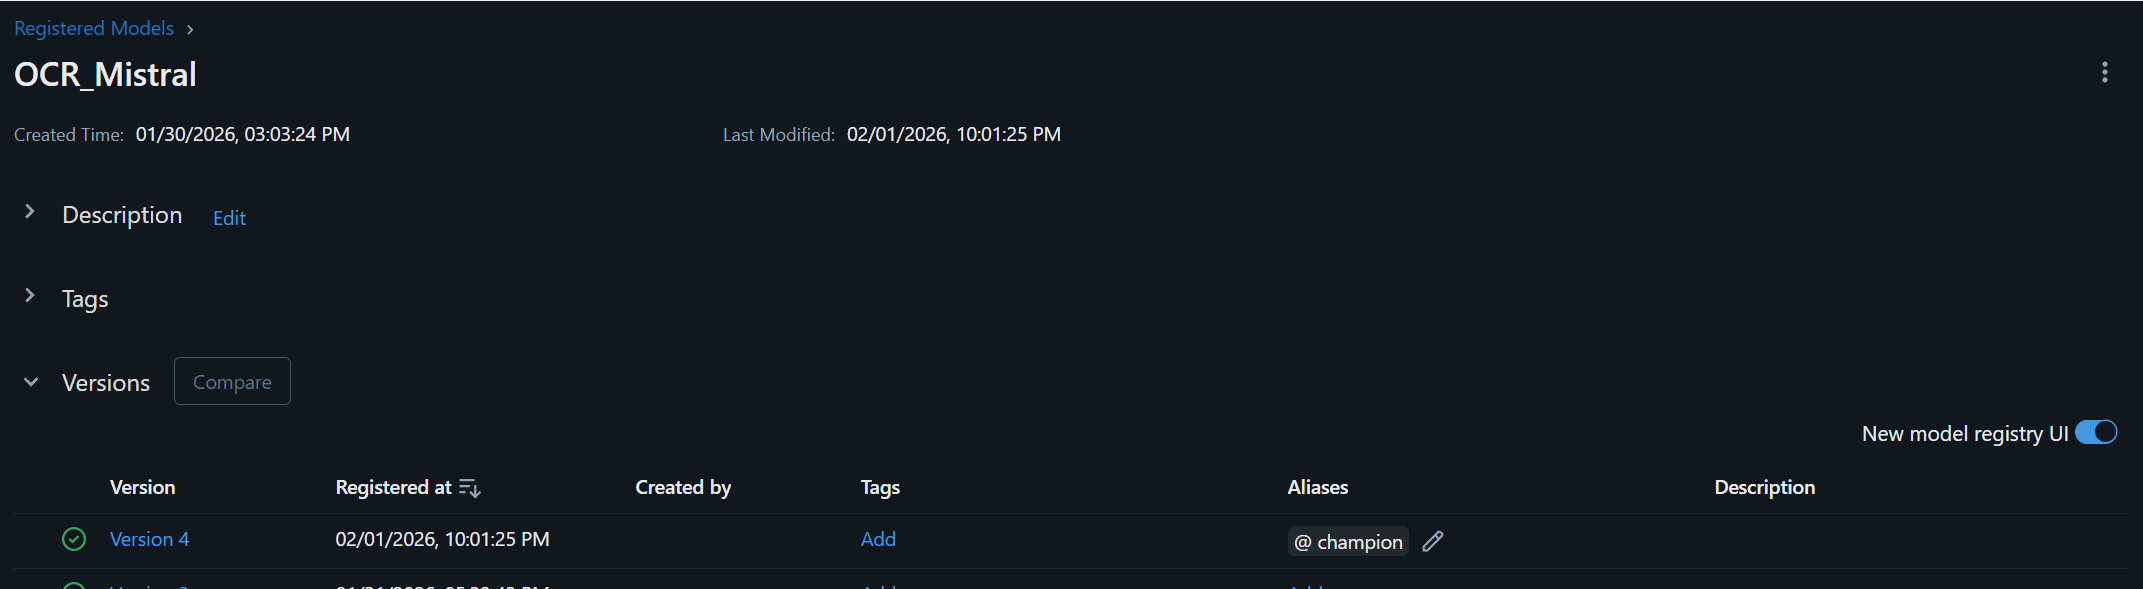
\includegraphics[keepaspectratio]{images/mlflow_modele.png}}
\emph{(Image attendue : Capture d'écran montrant le Model Registry dans
MLflow avec un modèle tagué ``Champion'')}

\section{Structure Technique du Code
Source}\label{structure-technique-du-code-source}

Avant de détailler l'API, il est essentiel de comprendre l'organisation
modulaire du code dans le dépôt \texttt{src/ocr\_comparison/}.


\includegraphics[width=20.22in,height=3.15in]{mise_en_production_files/figure-latex/mermaid-figure-3.png}

\subsection{Fonctions Clés par
Module}\label{fonctions-cluxe9s-par-module}

\begin{longtable}[]{@{}
  >{\raggedright\arraybackslash}p{(\linewidth - 4\tabcolsep) * \real{0.3333}}
  >{\raggedright\arraybackslash}p{(\linewidth - 4\tabcolsep) * \real{0.3333}}
  >{\raggedright\arraybackslash}p{(\linewidth - 4\tabcolsep) * \real{0.3333}}@{}}
\toprule\noalign{}
\begin{minipage}[b]{\linewidth}\raggedright
Module
\end{minipage} & \begin{minipage}[b]{\linewidth}\raggedright
Fonction Principale
\end{minipage} & \begin{minipage}[b]{\linewidth}\raggedright
Rôle
\end{minipage} \\
\midrule\noalign{}
\endhead
\bottomrule\noalign{}
\endlastfoot
\texttt{preprocessing\_all.py} & \texttt{apply\_preprocessing()} &
Applique les filtres OpenCV optimisés (CLAHE, Deskew). \\
\texttt{mistral\_model.py} & \texttt{extract\_invoice\_data()} & Appelle
l'API Mistral avec le prompt structuré. \\
\texttt{evaluations2.py} & \texttt{evaluate\_extraction()} & Compare les
prédictions avec le Ground Truth via métriques rigoureuses. \\
\texttt{ocr\_pipeline.py} & Classe \texttt{OCRPipeline} & Wrapper MLflow
héritant de \texttt{PythonModel} pour le versioning. \\
\end{longtable}

\section{Développement de l'API
REST}\label{duxe9veloppement-de-lapi-rest}

\subsection{Architecture FastAPI +
MLflow}\label{architecture-fastapi-mlflow}

L'API a été conçue pour être \textbf{agnostique du modèle}, permettant
de changer de version sans redéployer le code.

\subsubsection{Chargement Dynamique des
Modèles}\label{chargement-dynamique-des-moduxe8les}

\begin{Shaded}
\begin{Highlighting}[]
\ImportTok{import}\NormalTok{ mlflow.pyfunc}

\CommentTok{\# Cache pour éviter les rechargements}
\NormalTok{MODELS\_CACHE }\OperatorTok{=}\NormalTok{ \{\}}

\AttributeTok{@app.post}\NormalTok{(}\StringTok{"/predict\_mlflow"}\NormalTok{)}
\ControlFlowTok{async} \KeywordTok{def}\NormalTok{ predict\_mlflow(}\BuiltInTok{file}\NormalTok{: UploadFile, model\_uri: }\BuiltInTok{str}\NormalTok{):}
    \ControlFlowTok{if}\NormalTok{ model\_uri }\KeywordTok{not} \KeywordTok{in}\NormalTok{ MODELS\_CACHE:}
\NormalTok{        MODELS\_CACHE[model\_uri] }\OperatorTok{=}\NormalTok{ mlflow.pyfunc.load\_model(model\_uri)}
    
\NormalTok{    model }\OperatorTok{=}\NormalTok{ MODELS\_CACHE[model\_uri]}
\NormalTok{    results }\OperatorTok{=} \ControlFlowTok{await}\NormalTok{ run\_in\_threadpool(}\KeywordTok{lambda}\NormalTok{: model.predict([file\_path]))}
    \ControlFlowTok{return}\NormalTok{ \{}\StringTok{"results"}\NormalTok{: results\}}
\end{Highlighting}
\end{Shaded}

\subsubsection{Gestion de
l'Asynchronisme}\label{gestion-de-lasynchronisme}

L'utilisation de \texttt{nest\_asyncio} permet d'exécuter des boucles
événementielles imbriquées, nécessaire car certains modèles utilisent
\texttt{asyncio.run()} en interne.

\subsection{Contrat d'Interface
(Pydantic)}\label{contrat-dinterface-pydantic}

La validation stricte des schémas garantit que le JSON retourné est
conforme à l'ERP client.

\begin{Shaded}
\begin{Highlighting}[]
\KeywordTok{class}\NormalTok{ InvoiceItem(BaseModel):}
\NormalTok{    description: }\BuiltInTok{str}
\NormalTok{    quantity: Optional[}\BuiltInTok{int}\NormalTok{]}
\NormalTok{    amount: }\BuiltInTok{float}

\KeywordTok{class}\NormalTok{ InvoiceResponse(BaseModel):}
\NormalTok{    invoice\_id: }\BuiltInTok{str}
\NormalTok{    date: date}
\NormalTok{    items: List[InvoiceItem]}
\end{Highlighting}
\end{Shaded}

\pandocbounded{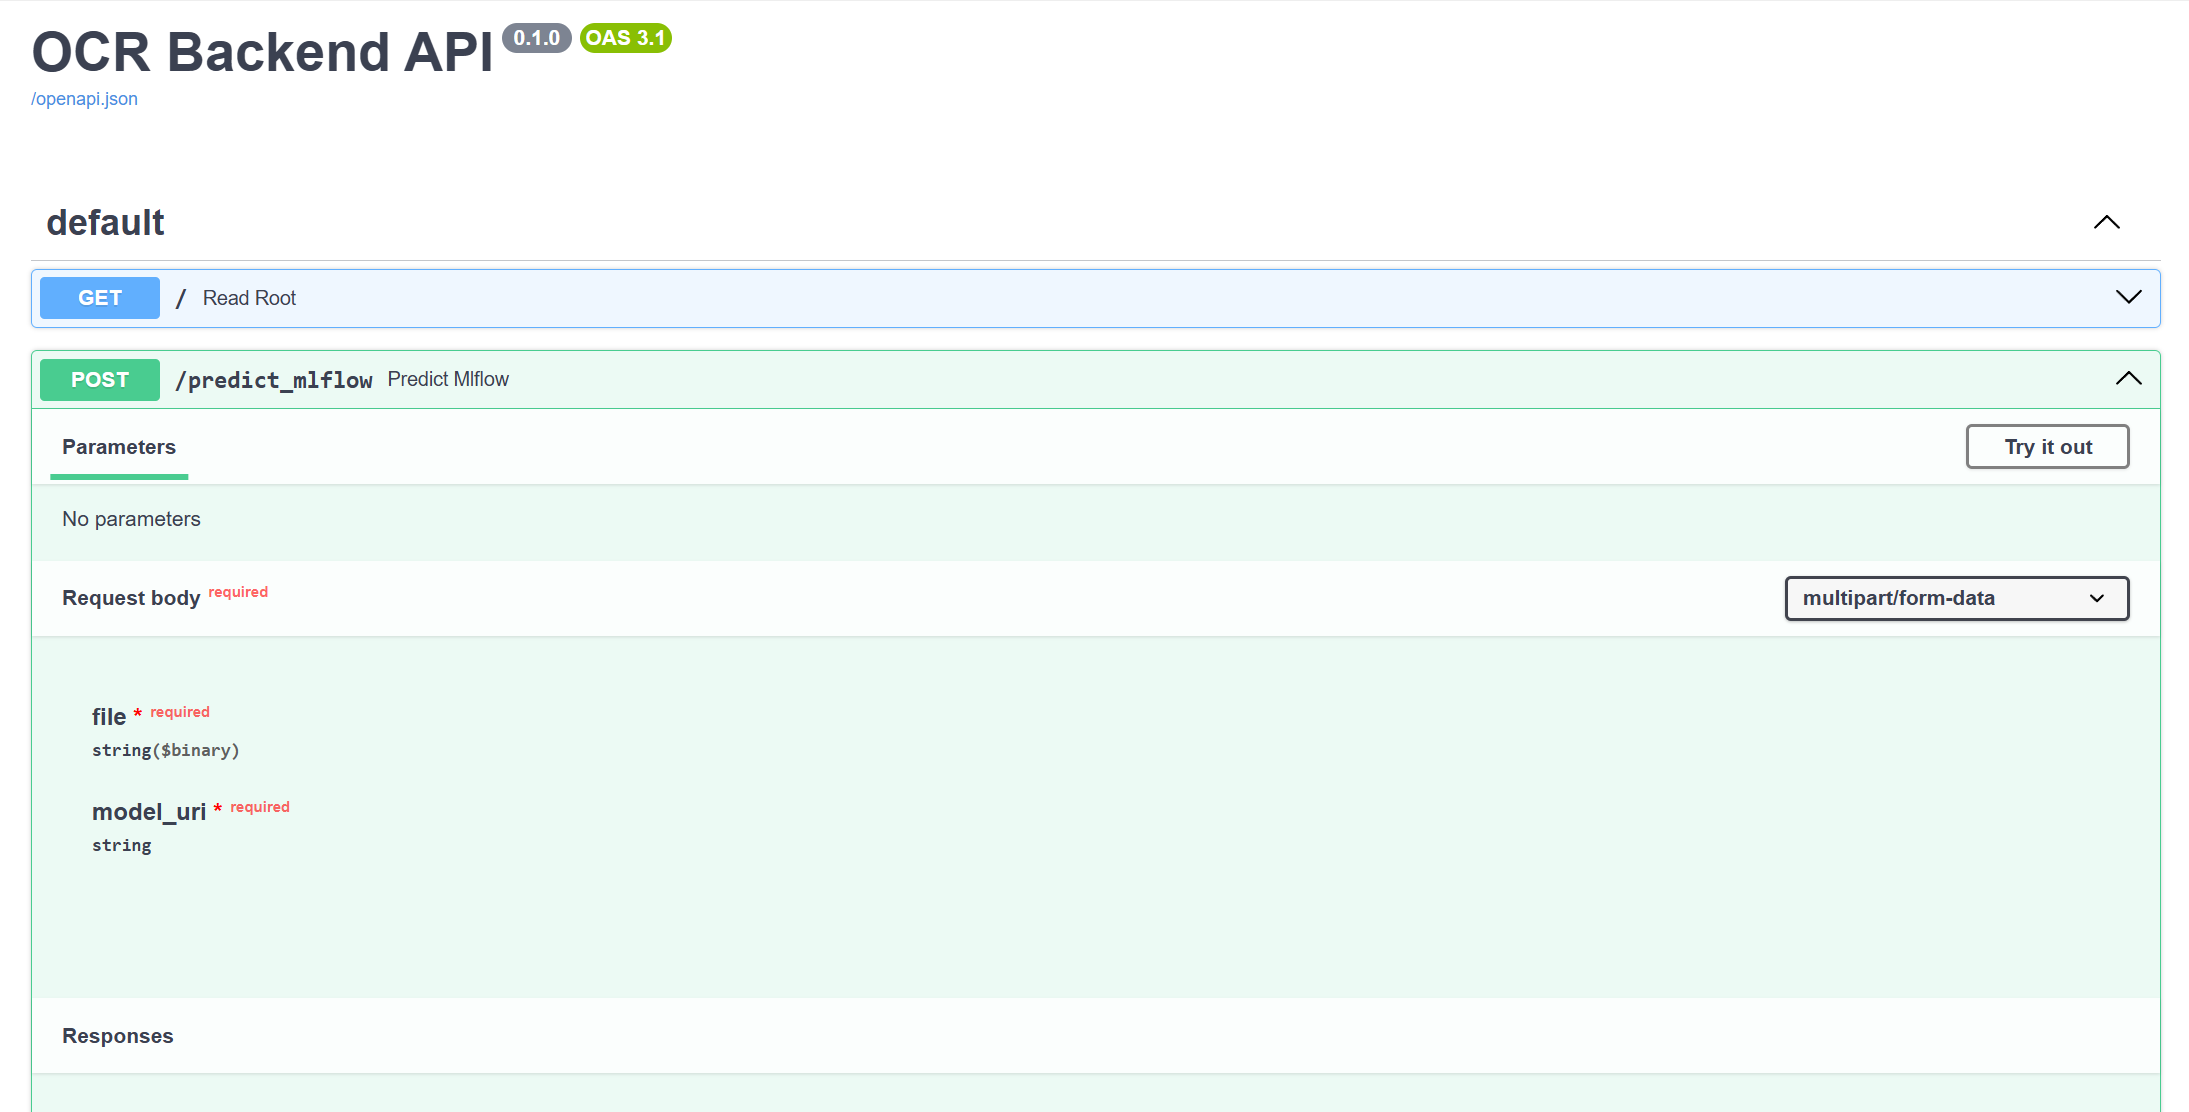
\includegraphics[keepaspectratio]{images/fastapi_mlflow.png}}
\emph{(Image attendue : Capture d'écran de l'interface /docs de FastAPI
montrant les endpoints disponibles)}

\section{Intégration dans l'Application
Streamlit}\label{intuxe9gration-dans-lapplication-streamlit}

L'application Streamlit existante a été enrichie pour consommer les
résultats de l'API.

\subsection{Flux d'Intégration}\label{flux-dintuxe9gration}


\includegraphics[width=11.47in,height=5.45in]{mise_en_production_files/figure-latex/mermaid-figure-2.png}

\subsection{Interface Multi-Pages}\label{interface-multi-pages}

L'application a été restructurée en pages indépendantes :

\begin{itemize}
\tightlist
\item
  \textbf{Upload \& Inference} : Envoi de documents et affichage des
  résultats.
\item
  \textbf{Model Comparison} : Tableau comparatif Pandas filtrable par
  champs.
\item
  \textbf{MLflow Dashboard} : Visualisation des runs directement dans
  Streamlit.
\end{itemize}

\pandocbounded{
\includegraphics[keepaspectratio]{images/app_inference.png}}
\emph{(Image attendue : Capture d'écran de l'application Streamlit
affichant une facture et les données extraites à côté)}

\section{Stratégie de Monitoring et
Tests}\label{stratuxe9gie-de-monitoring-et-tests}

\subsection{Métriques d'Évaluation
Rigoureuses}\label{muxe9triques-duxe9valuation-rigoureuses}

Pour garantir la qualité du système, plusieurs métriques complémentaires
ont été implémentées.

\subsubsection{Métriques au Niveau
Document}\label{muxe9triques-au-niveau-document}

\begin{itemize}
\tightlist
\item
  \textbf{Exact Match Rate (EMR)} : Pourcentage de champs (invoice\_id,
  date) parfaitement extraits.
\item
  \textbf{Accuracy} : Proportion globale de champs corrects.
\end{itemize}

\subsubsection{Métriques au Niveau
Texte}\label{muxe9triques-au-niveau-texte}

\begin{itemize}
\tightlist
\item
  \textbf{CER (Character Error Rate)} : Distance de Levenshtein
  normalisée au niveau caractère.
\item
  \textbf{WER (Word Error Rate)} : Distance au niveau mot, sensible aux
  erreurs de tokenisation.
\end{itemize}

\subsubsection{Métriques au Niveau Structurel (Line
Items)}\label{muxe9triques-au-niveau-structurel-line-items}

\begin{itemize}
\tightlist
\item
  \textbf{Recall} : Proportion d'articles réellement présents qui ont
  été détectés.
\item
  \textbf{Precision} : Proportion d'articles détectés qui sont corrects.
\item
  \textbf{F1-Score avec Fuzzy Matching} : Utilisation de
  \texttt{RapidFuzz} pour tolérer les variantes orthographiques (``Câble
  AISG'' vs ``Cable AISG'').
\end{itemize}

\subsection{Défis d'Évaluation
Rencontrés}\label{duxe9fis-duxe9valuation-rencontruxe9s}

L'évaluation de documents semi-structurés comme les factures présente
des défis uniques :

\begin{enumerate}
\def\labelenumi{\arabic{enumi}.}
\item
  \textbf{Fragmentation} : Un article peut être décrit sur plusieurs
  lignes.
\item
  \textbf{Variabilité linguistique} : Multilinguisme (anglais, espagnol,
  chinois).
\item
  \textbf{Ambiguïté sémantique} : ``Total TTC'' vs ``Total'' vs ``Amount
  Due''.
\end{enumerate}

\subsubsection{Solution Adoptée}\label{solution-adoptuxe9e}

Un système de \textbf{matching par similarité sémantique} (Fuzzy Token
Ratio \textgreater{} 80\%) combiné à une validation de cohérence
numérique (montants dans ±5\%).

\subsection{Suivi MLflow en
Production}\label{suivi-mlflow-en-production}

Chaque inférence en production est tracée avec :

\begin{itemize}
\tightlist
\item
  \textbf{Temps de latence} (objectif : \textless{} 6s/facture).
\item
  \textbf{Coût par requête} (API Mistral vs Groq).
\item
  \textbf{Métrique de confiance} (score interne du modèle).
\end{itemize}

Les graphiques MLflow permettent de détecter toute \textbf{dérive de
performance} (Data Drift) lorsque de nouveaux formats de factures
apparaissent.

\subsubsection{Métriques Prioritaires (Alignées avec le
Business)}\label{muxe9triques-prioritaires-alignuxe9es-avec-le-business}

D'après les objectifs de l'entreprise (SLA \textless{} 5min, précision
\textgreater{} 90\%), les métriques suivantes sont surveillées en
priorité :

\begin{enumerate}
\def\labelenumi{\arabic{enumi}.}
\tightlist
\item
  \textbf{F1-Score global} : Indicateur principal de qualité.
\item
  \textbf{Latence P95} : 95\% des requêtes doivent respecter le SLA.
\item
  \textbf{Coût par 1000 factures} : Pour valider la rentabilité vs
  Document AI.
\end{enumerate}

\pandocbounded{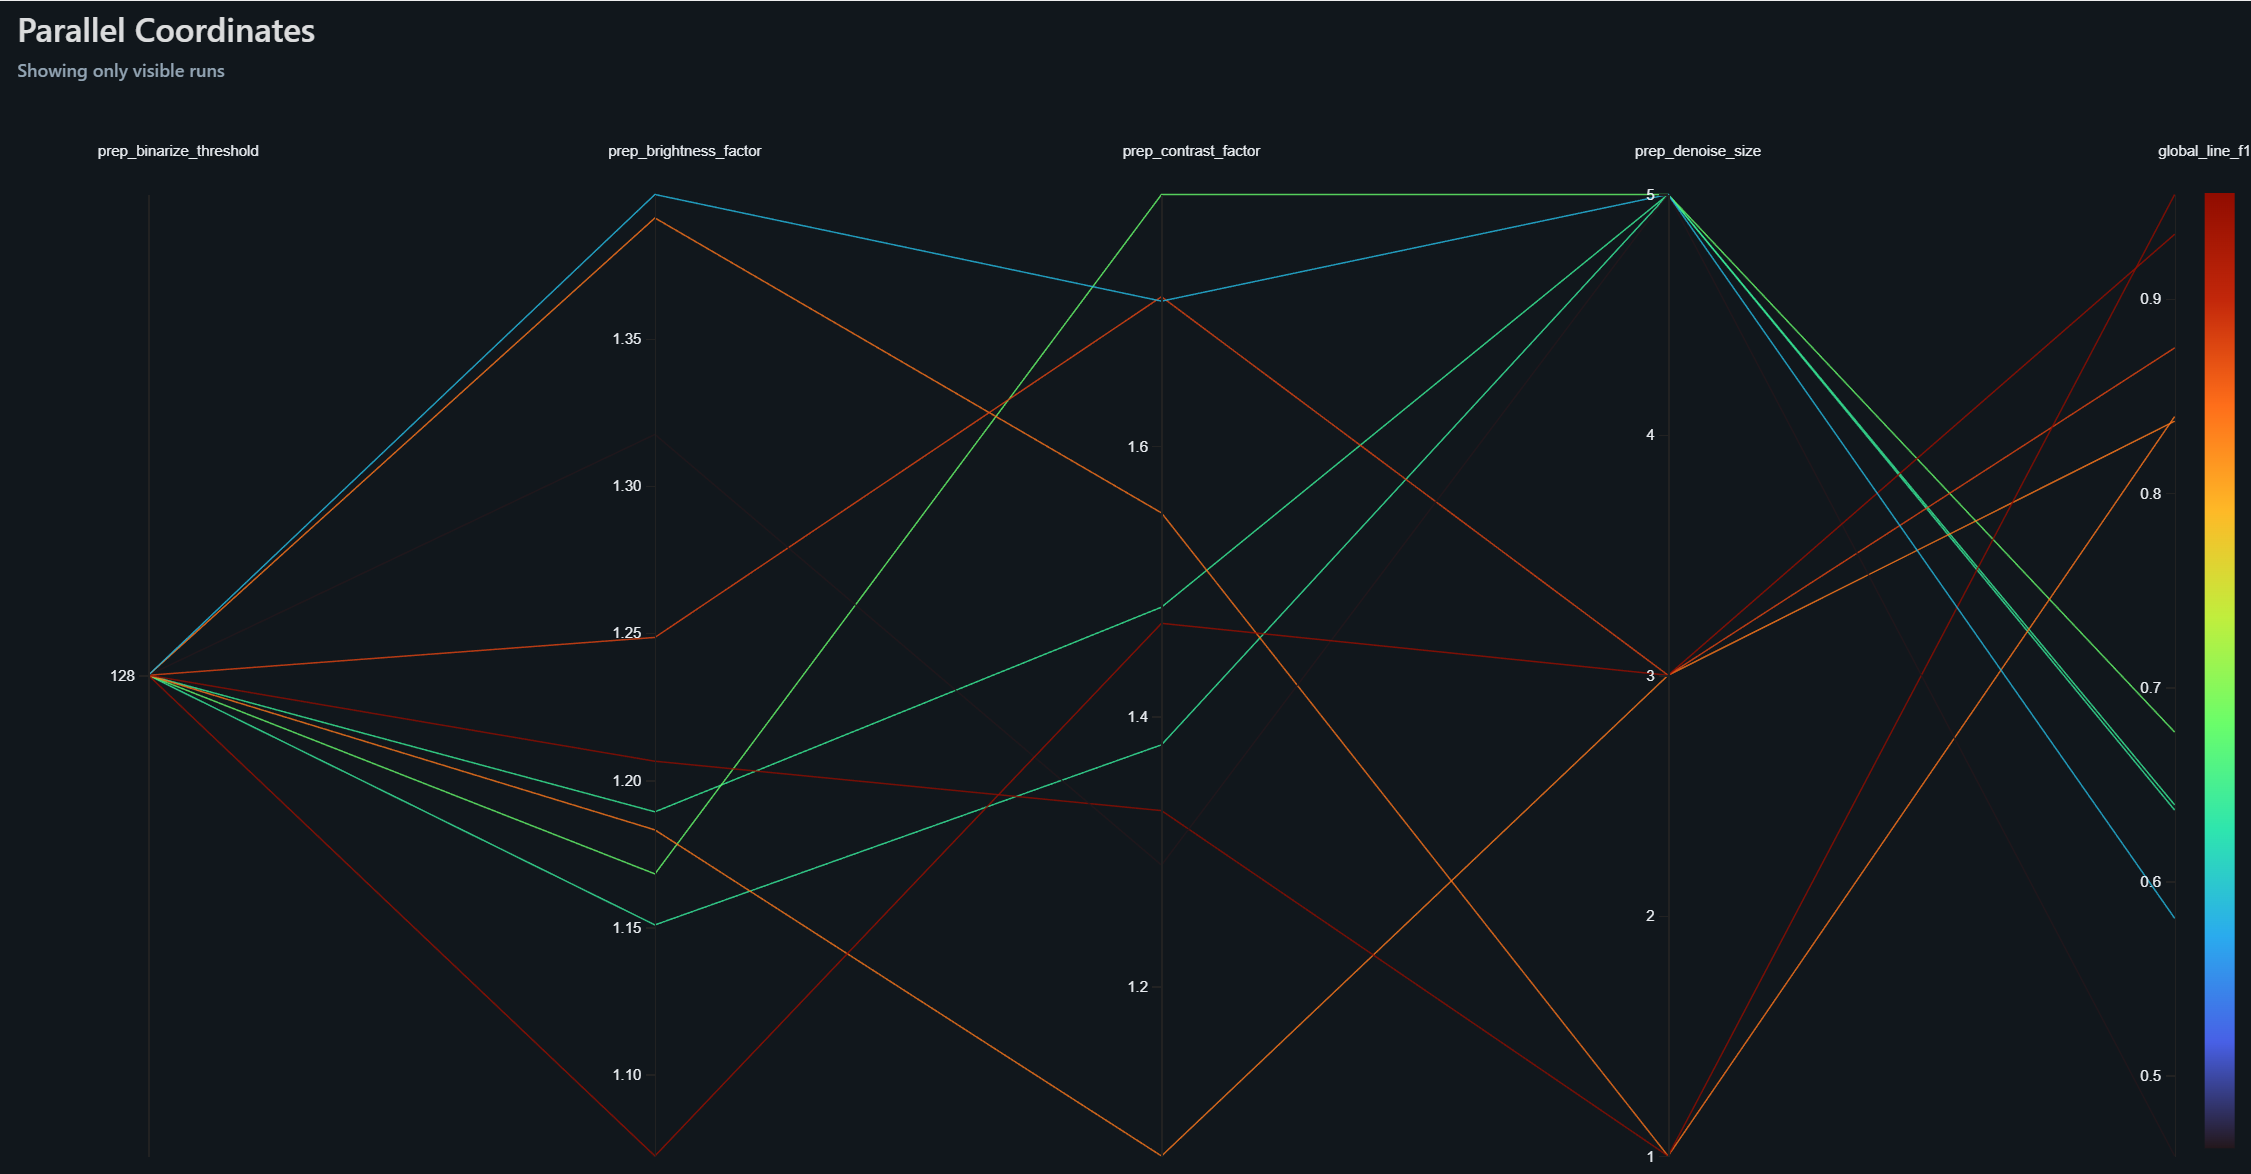
\includegraphics[keepaspectratio]{images/line_f1_optimal.png}}
\emph{(Image attendue : Graphique MLflow comparant le F1-Score de
plusieurs runs expérimentaux)}

\subsection{Étapes Techniques}\label{uxe9tapes-techniques}

\begin{enumerate}
\def\labelenumi{\arabic{enumi}.}
\item
  \textbf{Build} : Création de l'image Docker via le
  \texttt{Dockerfile.backend}.
\item
  \textbf{Tests Automatisés} : Exécution de \texttt{evaluations2.py} sur
  un jeu de validation.
\item
  \textbf{Déploiement GCP} : Poussée vers Cloud Run
\item
  \textbf{Monitoring Post-Déploiement} : Vérification des métriques de
  santé (Uptime, Error Rate).
\end{enumerate}

\subsection{Infrastructure as Code
(Terraform)}\label{infrastructure-as-code-terraform}

Les ressources GCP sont déclarées dans des fichiers \texttt{.tf} :

\begin{itemize}
\tightlist
\item
  \textbf{GCS Bucket} pour les documents entrants.
\item
  \textbf{Service Account} avec permissions MLflow.
\item
  \textbf{Cloud Run Service} avec auto-scaling.
\end{itemize}

Cela garantit que l'environnement peut être recréé identiquement en cas
de migration.

\section{Démonstration du Système
Complet}\label{duxe9monstration-du-systuxe8me-complet}

La soutenance inclura une démonstration en direct couvrant :

\begin{enumerate}
\def\labelenumi{\arabic{enumi}.}
\tightlist
\item
  \textbf{Upload d'une facture} via Streamlit.
\item
  \textbf{Appel de l'API FastAPI} et inspection du JSON retourné.
\item
  \textbf{Consultation de MLflow} pour visualiser les métriques de cette
  inférence.
\item
  \textbf{Trigger d'un déploiement} via Git Push (si le temps le
  permet).
\end{enumerate}

\section{Ressources
Complémentaires}\label{ressources-compluxe9mentaires}

Une documentation technique extensive du dépôt a été générée via une IA
spécialisée (DeepWiki). Elle détaille la structure des paquets et les
stratégies de prétraitement (Baseline, Intelligent, Comprehensive).

\begin{quote}
{[}WARNING{]} Cette documentation est générée automatiquement par IA et
peut contenir des approximations mineures, mais elle offre une vue
exhaustive de l'architecture du code.
\end{quote}

\begin{itemize}
\tightlist
\item
  \textbf{Lien vers la Wiki} :
  \url{https://deepwiki.com/jeanluissoto/ocr_pipeline}
\end{itemize}

\section{Retour à la Partie 1}\label{retour-uxe0-la-partie-1}

Si vous avez manqué la sélection du modèle et l'optimisation des
paramètres, vous pouvez revenir à la première partie :

\href{index.qmd}{Partie 1/2 : Sélection et Paramétrage}

\section{Conclusion}\label{conclusion}

Ce projet illustre la mise en production complète d'un service d'IA, du
développement de l'API à l'intégration dans une application métier, en
passant par un système de monitoring robuste et une chaîne CI/CD
automatisée. L'architecture choisie permet non seulement de satisfaire
les besoins actuels mais offre également la flexibilité nécessaire pour
les évolutions futures.




\end{document}
